\begin{figure*}[hbtp]
  \centering
  \subfigure{
    \label{fig:leiden-pass--all}
    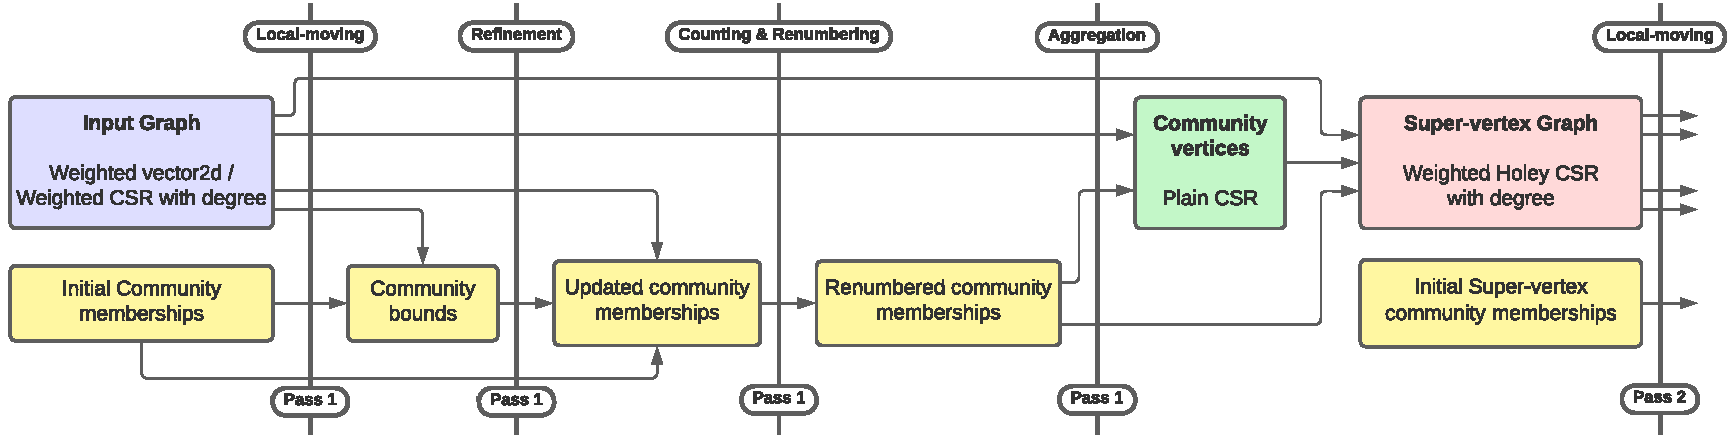
\includegraphics[width=0.98\linewidth]{out/leiden-pass.pdf}
  } \\[-2ex]
  \caption{A flow diagram illustrating the first pass of GVE-Leiden for either a Weighted 2D-vector-based or a Weighted CSR with degree-based input graph. In the local-moving phase, vertex community memberships are updated to obtain community bounds for the refinement phase, until the cumulative delta-modularity change across all vertices reaches a specified threshold. Then, in the refinement phase, the each vertex starts in a singleton community, and community memberships are updated similarly to the local-moving phase, with vertices changing communities within their bounds. These community memberships are then counted and renumbered. In the aggregation phase, community vertices in a CSR are first obtained. This is used to create the super-vertex graph stored in a Weighted Holey CSR with degree. Subsequent passes use a Weighted Holey CSR with degree and initial community memberships for super-vertices from the previous pass as input.}
  \label{fig:leiden-pass}
\end{figure*}
